\chapter{序論}
欧州原子力研究機構(\textbf{CERN})に設置されている大型ハドロン衝突型加速器(\textbf{LHC})では、現在、素粒子物理学の基礎となっている標準模型の精密測定や標準模型を超える物理現象の探索が行われている。
ATLAS実験はLHC上にある4つの衝突点の1つで行われている実験であり、ATLAS検出器を用いて生成粒子の測定が行われている。LHCでは加速器のアップグレード(\textbf{HL-LHC})を予定しており、これに向けてATLAS検出器のアップグレードを行う。この章ではLHC-ATLAS実験とそのアップグレード計画について説明する。

\section{素粒子標準模型とその問題点}
\subsection{素粒子標準模型}
現在素粒子物理学で基礎となっており、多くの実験事実を説明している理論を「標準模型」\cite{1-9}と呼ぶ。
標準模型はスピン1/2のフェルミオンである6種類の「クォーク」と6種類の「レプトン」、スピン1の4種類の「ゲージボソン」及びスピン0の「ヒッグスボソン」から成る。
表\ref{SM_particle_fermion}、\ref{SM_particle_boson}に一覧を示す。
2012年7月にCERNで新粒子の発見が発表され、これがヒッグス粒子であると認定され標準模型における全ての素粒子が実験的に確認された。

自然界には電磁相互作用、強い相互作用、弱い相互作用、重力相互作用の4種類の相互作用がある。
標準模型は強い相互作用を記述する量子色力学(Quantum ChromoDynamics: QCD)、電磁相互作用と弱い相互作用を統一した電弱統一理論(Glashow-Weinberg-Salam: GWS)から成る。重力相互作用は標準理論では扱っていない。
強い相互作用は色荷(Color)を持ち、$SU(3)_C$の対称性を持つ。8種類の$g$によって力が媒介される。
電弱相互作用は$SU(2)_L \otimes U(1)_Y$の対称性を持つ。力を媒介する粒子として$W_1$、$W_2$、$W_3$と$B$が存在する。このうち$W_1、W_2$が混合して$W^{\pm}、W_3、B$が混合して$Z、\gamma$となる。

\begin{table}[tbp]
\begin{center}
\caption[標準模型のフェルミオン]{標準模型のフェルミオン。}
\label{SM_particle_fermion}
  \small
  \begin{tabular}{|l|lll|lll|} \hline
    世代 & クォーク & 電荷[$e$] & 質量[MeV/$c^2$]    & レプトン    & 電荷[$e$]   & 質量[MeV/$c^2$]      \\ \hline \hline
    1    & $u$      & $2/3$     & $〜2.3$            & $e^-$       & $-1$        & $0.511$              \\
         & $d$      & $-1/3$    & $〜4.8$            & $\nu_e$     & $0$         & $<2.2\times 10^{-6}$ \\ \hline
    2    & $c$      & $2/3$     & $〜1280$           & $\mu^-$     & $-1$        & $105.7$              \\
         & $s$      & $-1/3$    & $〜95$             & $\nu_\mu$   & $0$         & $<0.19$              \\ \hline
    3    & $t$      & $2/3$     & $〜1.73\times10^5$ & $\tau^-$    & $-1$        & $1777$               \\
         & $b$      & $-1/3$    & $〜4200$           & $\nu_\tau$  & $0$         & $<18$                \\ \hline
  \end{tabular}
\end{center}
\end{table}

\begin{table}[tbp]
\begin{center}
\caption[標準模型のボソン]{標準模型のボソン。}
\label{SM_particle_boson}
  \small
  \begin{tabular}{|llllll|} \hline
    記号      & 名称           & 相互作用 & スピン    & 電荷[$e$] & 質量[GeV/$c^2$] \\ \hline
    $\gamma$  & 光子           & 電磁     & $1$       & $0$       & $0$             \\
    $W^{\pm}$ & 荷電弱ボソン   & 弱       & $1$       & $\pm 1$   & $80.4$          \\
    $Z$       & 中性弱ボソン   & 弱       & $1$       & $0$       & $91.2$          \\
    $g$       & グルーオン     & 強       & $1$       & $0$       & $0$             \\ \hline
    $H$       & ヒッグスボソン & -        & $0$       & $0$       & $125$           \\ \hline
  \end{tabular}
\end{center}
\end{table}

\subsection{ヒッグス機構と結合定数}

ここではヒッグス機構と結合定数について説明する\cite{1-12}。
標準模型のラグランジアンに質量項を導入すると、ゲージ不変性を破ってしまう。
これは素粒子が実際に質量を持つ事実と矛盾する。
ここで標準模型がゲージ不変性を保ちながら素粒子が質量を持つために、標準模型のラグランジアンにヒッグスセクターを導入する。
ここで導入するヒッグスセクターは複素スカラー場(ヒッグス場)$\phi$を用いて以下とする。
\bbb
\label{higgs_sector}
\mathcal{L}_{\rm Higgs} &=&  \left( \partial_\mu \phi \right)^\dag \left( \partial^\mu \phi \right) - V(\phi) \\
\eee

ここでヒッグスポテンシャル$V(\phi)$は、ゲージ対称性とくりこみ可能性の要請の下で、以下のようにする。
\bbb
V(\phi)  &=& \mu^2 \phi^\dag \phi + \lambda \left( \phi^\dag \phi \right)^2
\eee

$\mu^2<0$のとき、ポテンシャルが図\ref{higgs_potential}のような形となる。

\begin{figure}[bpt]\centering
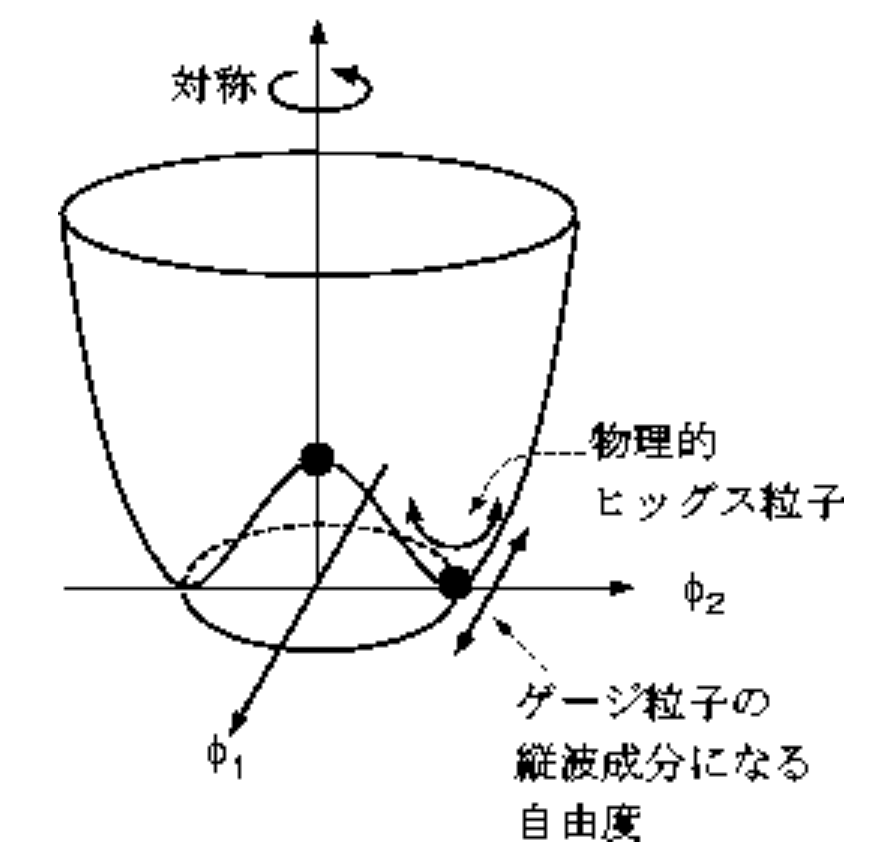
\includegraphics[width=6cm]{./higgs_potential.png}
\caption[ヒッグスポテンシャル]{ヒッグスポテンシャル\cite{1-13}。}
\label{higgs_potential}
\end{figure}

ポテンシャルが最小となる(真空)のは原点ではなく、図におけるリング状の領域である。
最小値となる点の中からある1つが選ばれ、その点が現在の真空となっている。これを「自発的対称性の破れ」と呼ぶ。
ゲージ粒子の質量は真空点の縦波成分となって現れ、これがヒッグス機構においてゲージ粒子が質量を獲得する原理となる。

ここで導入したヒッグスポテンシャル$V(\phi)$の特徴として、素粒子の質量とヒッグス粒子との結合定数が比例する。
真空期待値を$\left< \phi \right> =v/\sqrt{2}$とおくと、$W^{\pm}$、$Z$、フェルミオンとヒッグス粒子の結合の強さは以下のようになる。
\bbb
W^{\pm}:      &\frac{g^2}{2}v&    = \frac{e}{{\rm sin}\theta_W}m_W \\
Z:~           &\frac{(g')^2}{4}v& = \frac{2e}{{\rm sin}(2\theta_W)}m_Z \\
フェルミオン: &Y_f&               = \frac{\sqrt{2}}{v}m_f 
\eee
ここで$e$は素電荷、$\theta_W$はワインバーグ角と呼ばれる。
これらより、素粒子の質量とヒッグス粒子との結合定数が比例することが分かる。

これらの結合定数はLHCの実験で測定されており、線形性が見えている(図\ref{kappa_vs_mass})。
このヒッグスセクターの導入及び現在の標準模型は、実験事実と大きく矛盾していないことが分かる。

一方、ここで述べた標準模型におけるヒッグスセクターの導入は暫定的なものであり、任意性を持つ。
例えば、現在は複素スカラー場1つを導入しているが、複数の場を仮定することも可能である。
ヒッグス粒子の性質の精密測定によりこのヒッグスセクターの構造にせまることで、標準模型の検証をすることができる。

また標準模型を超える新理論ではしばしばこのヒッグスセクターの拡張を行い、標準理論における諸問題の説明を行っている。
この時、標準理論とは異なるヒッグス粒子の性質を導く場合がある。
ヒッグス粒子の精密測定は、標準模型を超える新理論にも影響を与える。

\begin{figure}[bpt]\centering
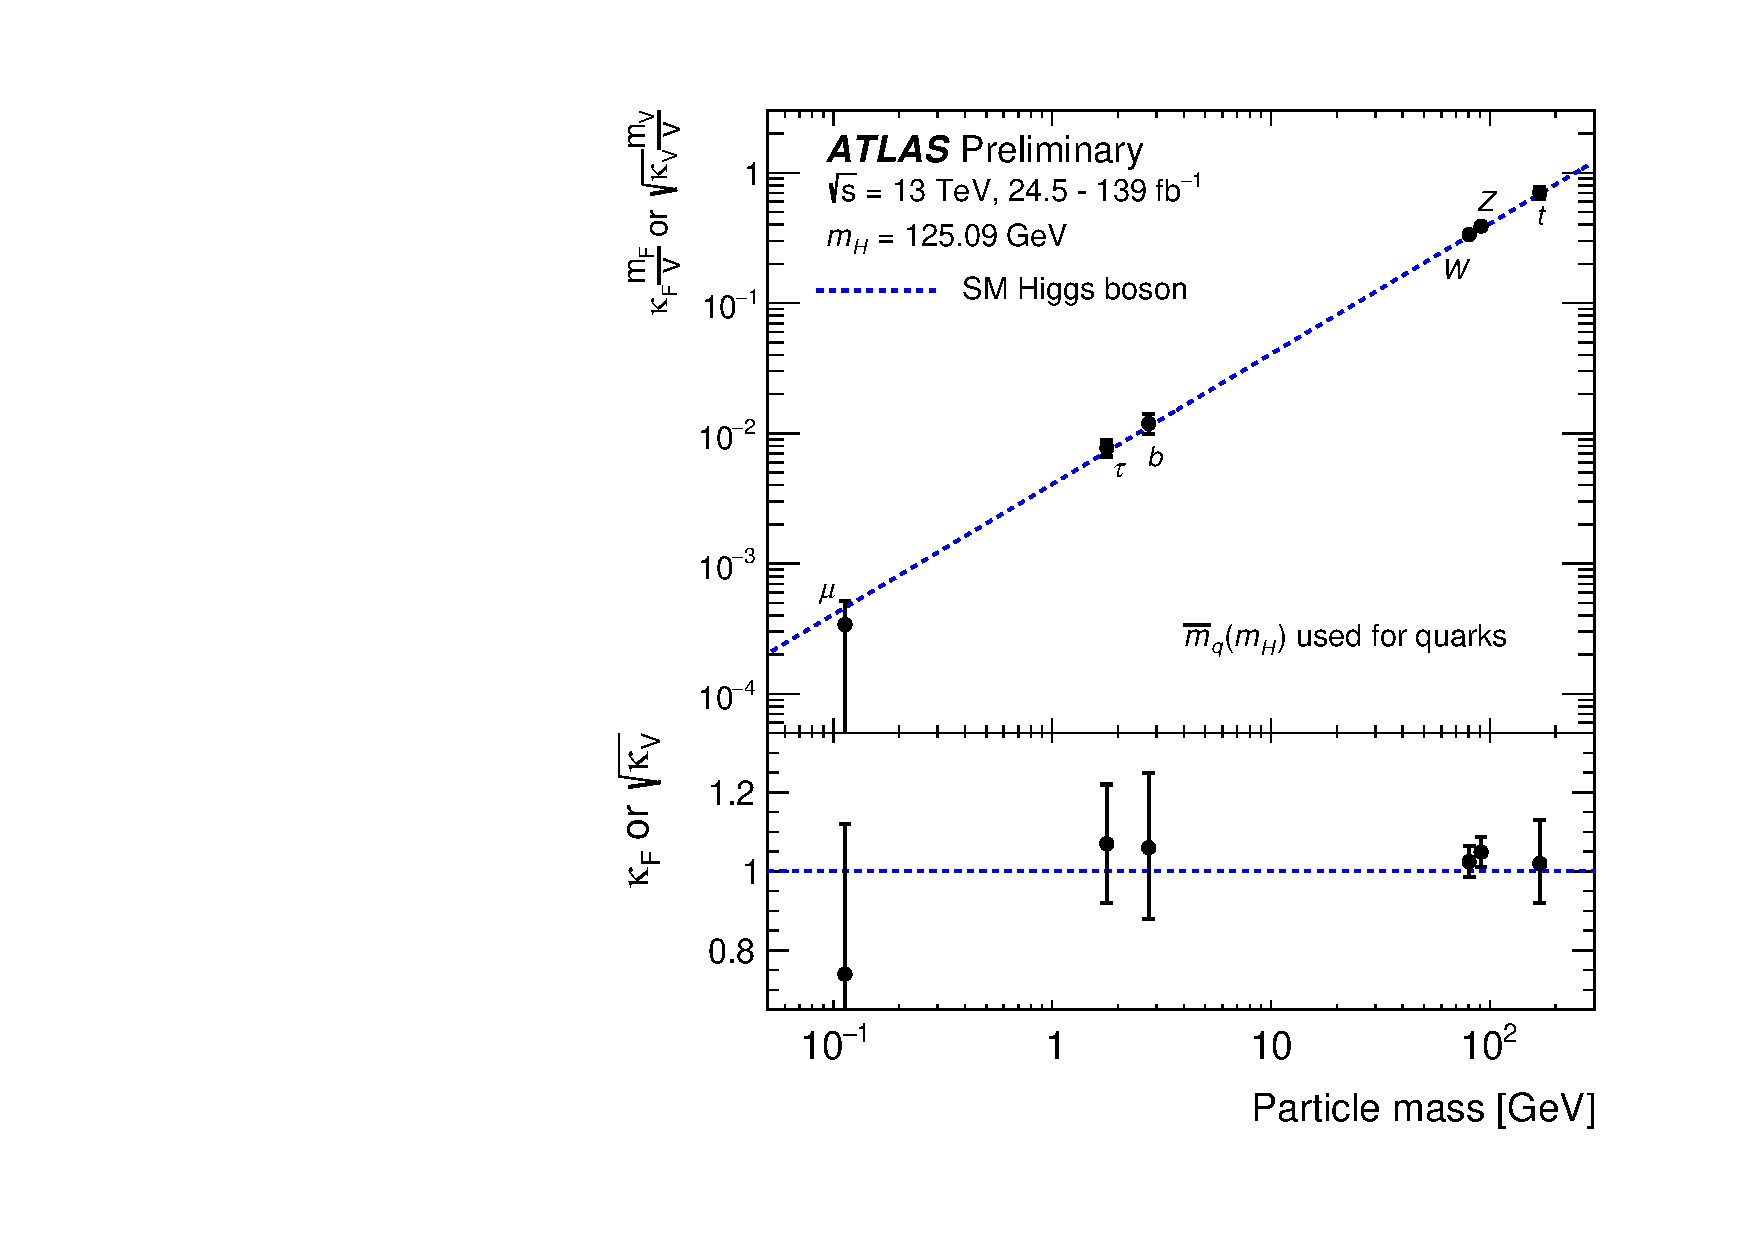
\includegraphics[width=10cm,angle=270]{./kappa_vs_mass.pdf}
\caption[標準模型の素粒子の質量とヒッグス粒子との結合定数の関係]{標準模型の素粒子の質量とヒッグス粒子との結合定数の関係\cite{1-10}。横軸は粒子の質量、縦軸は各粒子のヒッグス粒子との結合定数を示し、結合の強さを表す。各粒子の測定点が一直線状にのっており、線形性を示していることが分かる。}
\label{kappa_vs_mass}
\end{figure}

\subsection{問題点と新理論}
標準模型は、これまでの実験事実では説明できない以下の問題点を抱えている。
\begin{itemize}
  \item 重力理論との統一.
  \item なぜ素粒子は3世代なのか.
  \item 階層性問題.
  \item 強い相互作用におけるCP問題.
  \item 暗黒物質,エネルギー.
  \item ニュートリノの質量.
  \item バリオン数の非対称性.
\end{itemize}

現在上にあげた標準模型の諸問題を解くために以下のような理論が考案されている。
\begin{itemize}
  \item 超対称性.
  \item 余剰次元.
  \item テクニカラー.
  \item プレオン模型.
  \item アクシオン.
  \item シーソー機構.
\end{itemize}

上にあげた中から特に超対称性\cite{1-11}について簡単に説明する。
超対称性とはボソンとフェルミオンを入れ替える演算に対する対称性である。
つまり標準模型の各粒子に対応した、スピンが1/2だけ異なる超対称性粒子の存在を予言する理論である。
標準理論ではヒッグス場として1つの複素スカラー場を導入したが、超対称性を導入すると最低でも2つの場を必要とする。
この場合、8個の独立な成分が現れ、$(W^{\pm},Z)$に加えて$(H^{\pm},H^0,h^0,A^0)$が追加される。
観測時には電荷を持つ粒子、中性粒子がそれぞれ混合し、$(\widetilde{\chi}^{\pm}_{1,2})$、$(\widetilde{\chi}^{0}_{1,2,3,4})$となる。
超対称性は上にあげた問題点において、暗黒物質、階層性問題を説明できる可能性を持っている。



\clearpage
\section{LHCについて}
LHCはCERNの地下およそ100 $\rm{m}$に設置されている周長26.7 $\rm{km}$の大型ハドロン衝突型加速器である。
バンチと呼ばれる陽子のかたまりを7 $\rm{TeV}$まで加速し、衝突させる。世界最大エネルギーの加速器である。

陽子ビームの加速は4つの前段加速器を用いて行う。始めに水素ガス中の水素原子から電子を分離することで陽子を生成する。
その後最初の線形加速器(Linear Accelarator: LINAC)、陽子シンクロトロンブースター(Proton Synchrotron Booster: PSB)、陽子シンクロトロン(Proton Synchrotron: PS)、スーパー陽子シンクロトロン(Super Proton Synchrotron)で加速されたのちLHCに入射する。CERNにある加速器の概要を図\ref{LHC_overview}に示す。
LHCには4つの衝突点があり、それぞれALICE(A Large Ion Collider Experiment)、LHCb、CMS(Compact Muon Solenoid)、ATLAS(A
Troidal LHC Apparatus)実験が行われている。それぞれの衝突点には崩壊粒子の飛跡やエネルギーを測定するための検出器が設置されており、取得したデータを元に多様な物理解析が行われている。

\begin{figure}[bpt]\centering
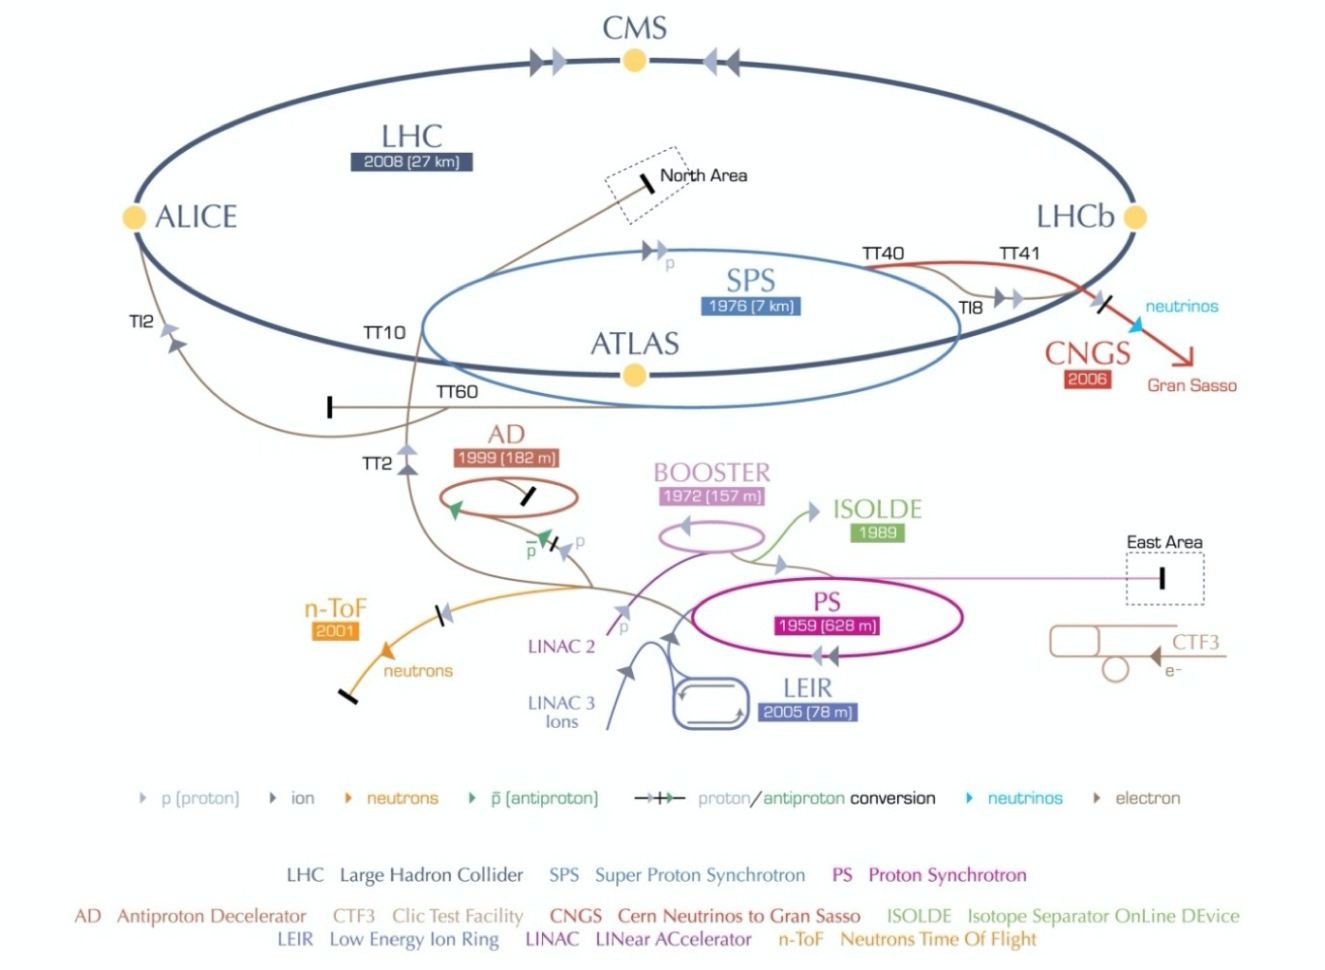
\includegraphics[width=12cm]{./LHC_overview.png}
\caption[加速器の全体像]{加速器の全体像\cite{1-1}。図はCERNに設置されている加速器の全体像を示す。陽子はいくつかの前段加速器で段階的に加速されLHCに入射する。LHC上には4つの衝突点が存在し、それぞれALICE、LHCb、CMS、ATLAS実験が行われている。}
\label{LHC_overview}
\end{figure}

\section{ATLAS実験}
初めにATLAS実験に用いる座標系と用語について説明する。まず衝突点を原点として右手座標系を定義しており、ビーム軸を$z$軸、これに対して垂直な平面を$x-y$平面とする。
$z$軸の正方向をSide-A、負方向をSide-Cと呼ぶ。
$x$軸方向は原点からみてLHCリングの中心に向かう方向であり、$y$軸は上に向かう方向である。
方位角$\phi$は$z$軸周りの角度であり、極角$\theta$は$z$軸とのなす角である。ATLAS実験では、極角$\theta$は以下のように擬ラピディティ$\eta$で表される。
また極角$\theta$と擬ラピディティ$\eta$の関係図を図\ref{eta_theta_graph}に示す。
\bbb
\eta = -\rm{ln \left( tan\left(\frac{\theta}{2}\right) \right) }
\label{eta_theta}
\eee

\begin{figure}[bpt]\centering
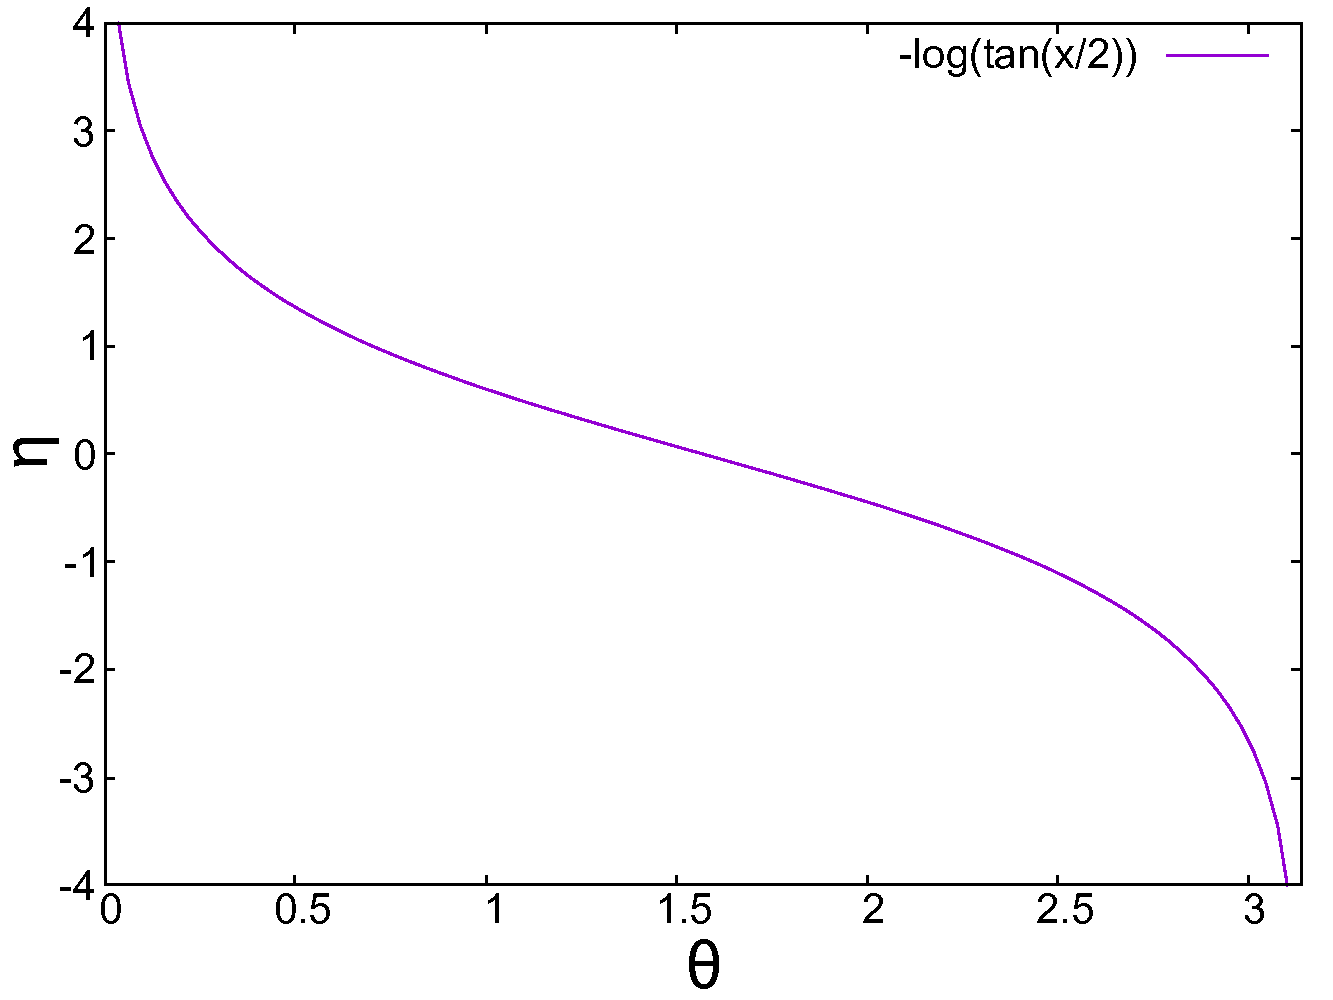
\includegraphics[width=6cm]{./data/eta_theta_relation.pdf}
\caption[極角$\theta$と擬ラピディティ$\eta$の関係図]{極角$\theta$と擬ラピディティ$\eta$の関係図。横軸は式\ref{eta_theta}における極角$\theta (0\leq\theta\leq\pi)$、縦軸は擬ラピディティ$\eta$を表している。図のように、$\eta$への変換により定義域が実数全体に広がる。}
\label{eta_theta_graph}
\end{figure}

\subsection{ATLAS検出器}
ATLAS検出器は複数の検出器から構成され、陽子の衝突によって生成された粒子の運動量、エネルギーを測定することができる。
最内層に内部飛跡検出器が設置されていて、次に超電導ソレノイド磁石、カロリメータ、トロイド磁石、ミューオン検出器の順に設置されている。
衝突点から見た立体角のほとんどを検出器で覆うような設計となっている。
ATLAS検出器の全体図を図\ref{atlas_detector}に示す。

\begin{figure}[bpt]\centering
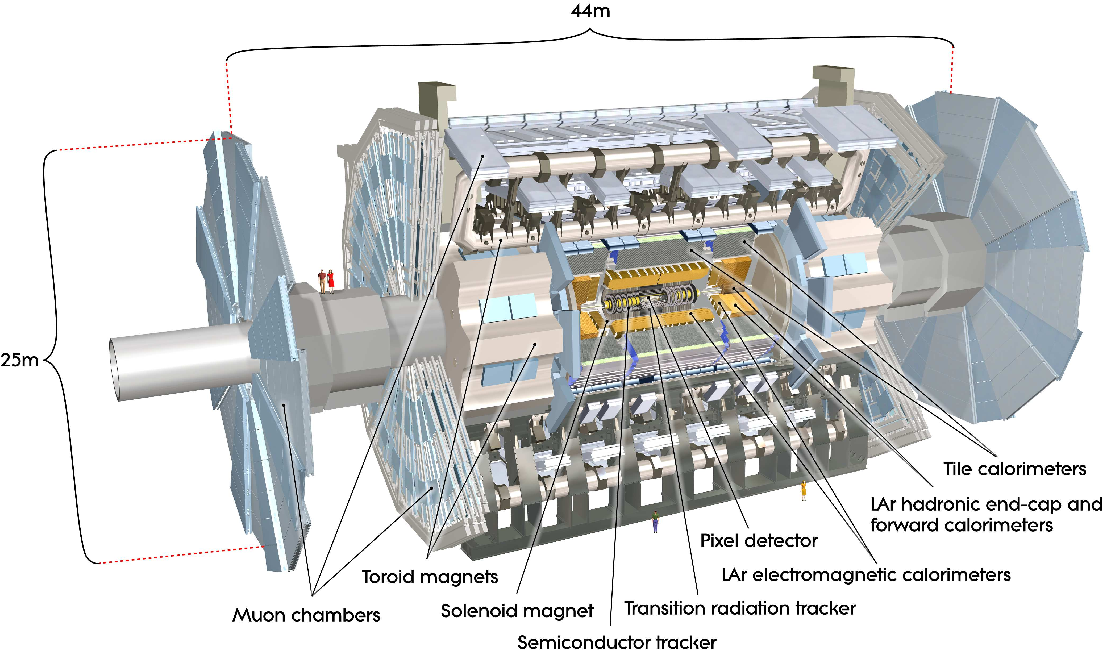
\includegraphics[width=10cm]{./atlas_detector.png}
\caption[ATLAS検出器の全体像]{ATLAS検出器の全体像\cite{1-2}。内側から内部飛跡検出器、ソレノイド磁石、カロリメータ、トロイド磁石、ミューオン検出器が設置されている。}
\label{atlas_detector}
\end{figure}

%\begin{figure}[bpt]\centering
%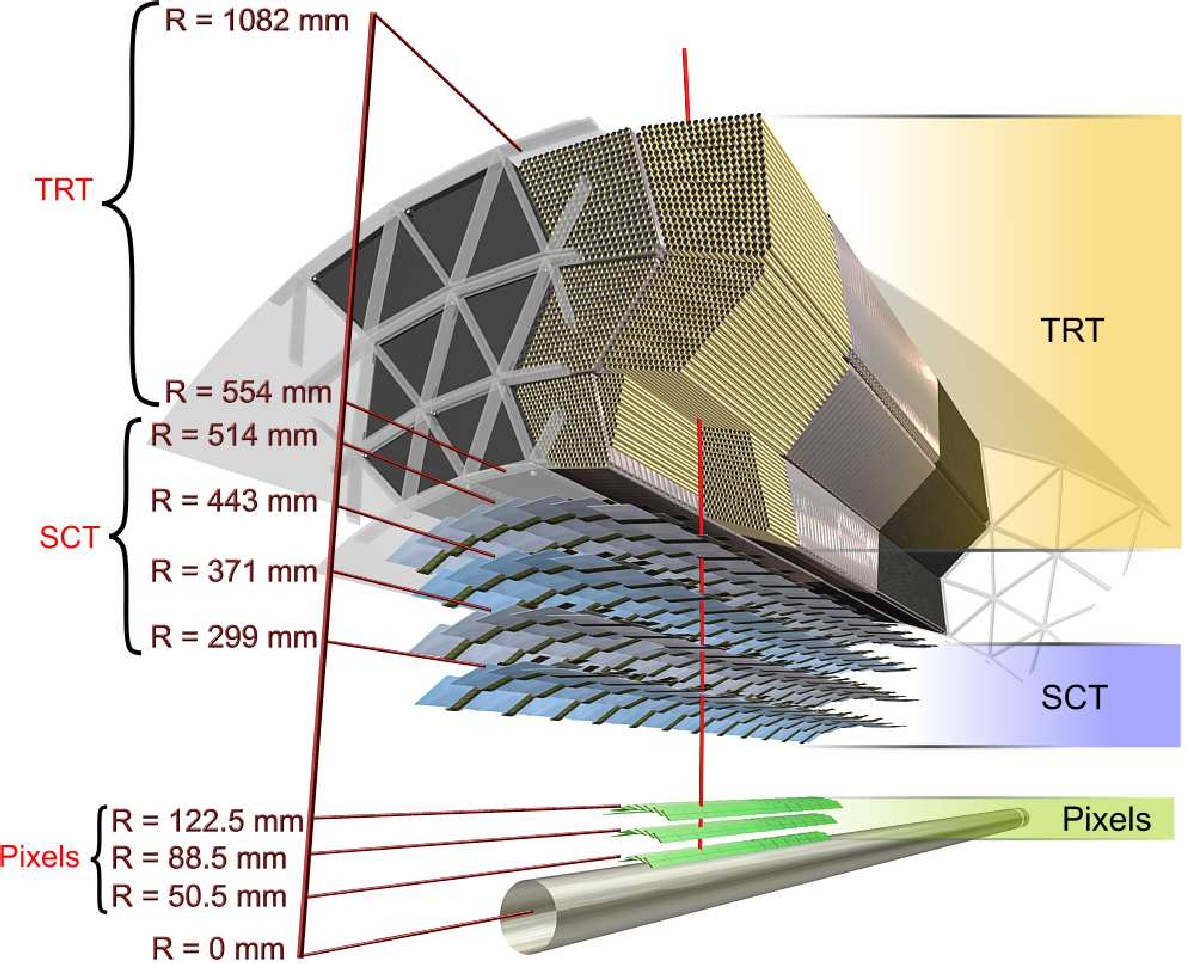
\includegraphics[width=10cm]{atlas_detector_cross_section}
%\caption[ATLAS検出器]{ATLAS検出器\cite{1-2}}
%\label{atlas_detector_cross_section}
%\end{figure}

\clearpage
\subsection{内部飛跡検出器}
ATLAS検出器の最内層に位置する検出器である。
内部飛跡検出器は粒子の飛跡測定をするための検出器であり、粒子の運動量や衝突点、崩壊点を計算する。
検出器の外側には超伝導ソレノイド磁石が設置されており、2 $\rm{T}$の磁場が$z$方向にかけられる。これにより荷電粒子はローレンツ力を受け、軌跡が曲がる。

内部飛跡検出器は3つの検出器で構成され、内側からピクセル検出器、ストリップ検出器、遷移放射検出器の順に設置されている。
ピクセル、ストリップ検出器は階層構造になっており、粒子は複数の検出器を通過する。
それぞれの検出器で取得した通過位置をつなぎ合わせることで粒子の飛跡を計算することができる。

内部飛跡検出器の全体図を図\ref{inner_detector}に示す。

\begin{figure}[bpt]\centering
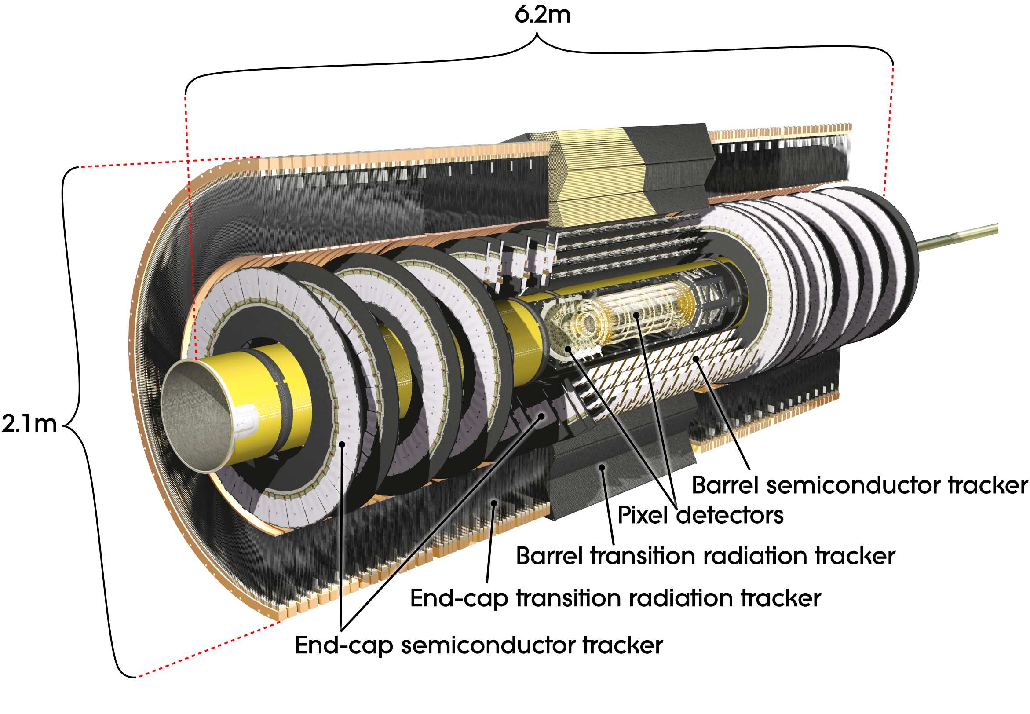
\includegraphics[width=10cm]{./inner_detector.png}
\caption[内部飛跡検出器の全体像]{内部飛跡検出器の全体像\cite{1-2}。内側からピクセル検出器、ストリップ検出器、遷移放射検出器が設置されている。また円筒状のバレル部とディスク上のエンドキャップ部を構造として持つ。}
\label{inner_detector}
\end{figure}


%検出器は$\eta$の範囲によってバレル部とエンドキャップ部に分かれる。図\ref{inner_cross_section}にビーム軸方向の端面図を示す。
%
%\begin{figure}[bpt]\centering
%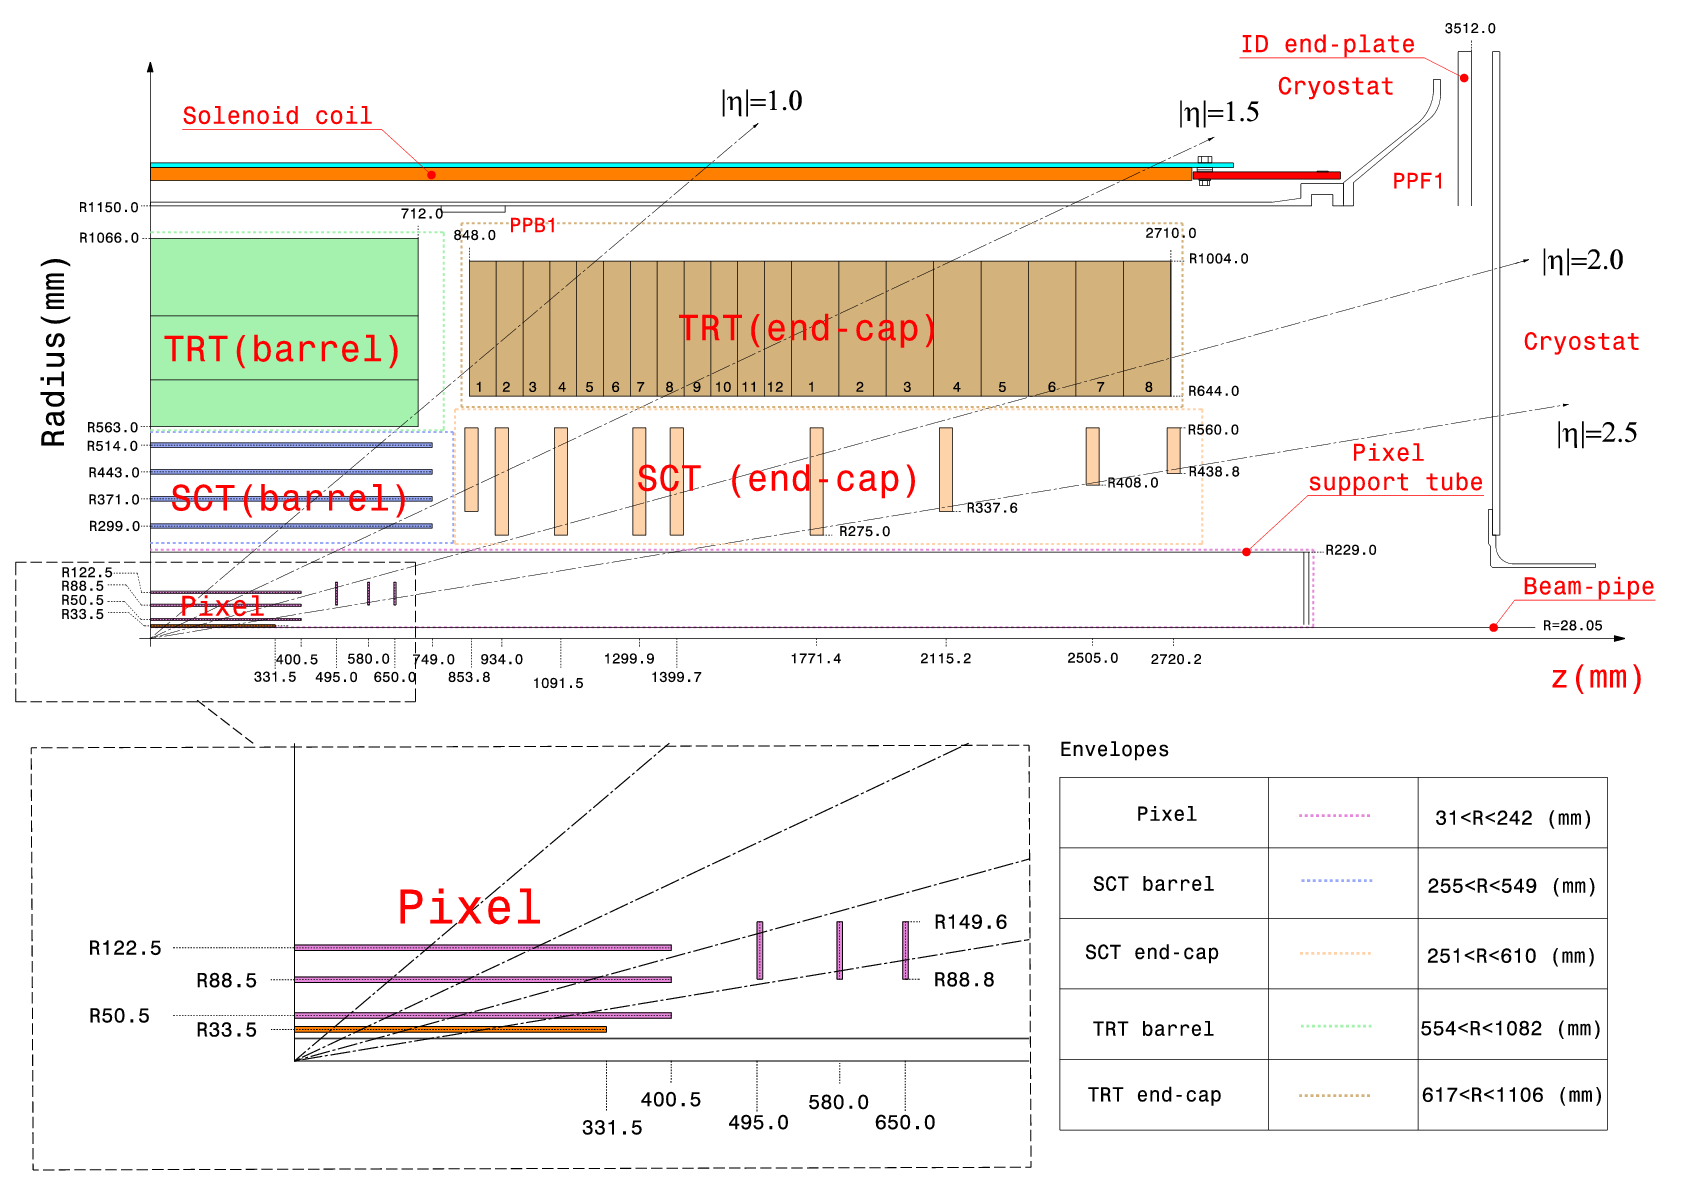
\includegraphics[width=12cm]{./inner_cross_section.png}
%\caption[内部飛跡検出器]{内部飛跡検出器\cite{1-4}}
%\label{inner_cross_section}
%\end{figure}

\subsubsection{ピクセル検出器}

内部飛跡検出器の最内層に位置する検出器である。
ピクセル検出器はバレル部が4層、エンドキャップ部が6層で構成される。
バレル部の最内層から順にIBL(Insertable B-Layer)、B-Layer、Layer-1、Layer-2と呼ばれる。

ピクセル検出器の全体図を図\ref{pixel_detector_overview}に示す。
\begin{figure}[bpt]\centering
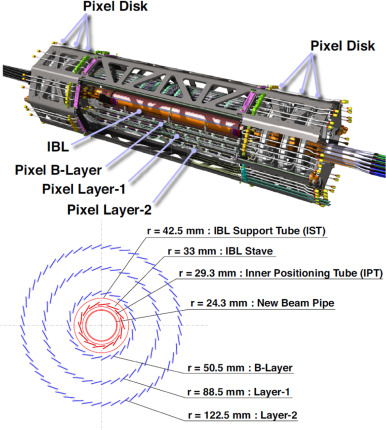
\includegraphics[width=8cm]{./pixel_detector_overview.jpg}
\caption[ピクセル検出器の全体像]{ピクセル検出器の全体像\cite{1-5}。上図はピクセル検出器の全体を模式的に表したものであり、下図はビーム軸方向から見たピクセル検出器の断面図である。バレル部の4層は内側からIBL、B-Layer、Layer-1、Layer-2と呼ぶ。}
\label{pixel_detector_overview}
\end{figure}

ピクセル検出器の各層は、モジュールと呼ばれる最小単位の検出器をいくつも搭載している。
ピクセルモジュールを図\ref{pixel_detector}に示す。
このピクセルモジュールの詳細については\ref{chap:pmodule}章で述べる。
\begin{figure}[bpt]\centering
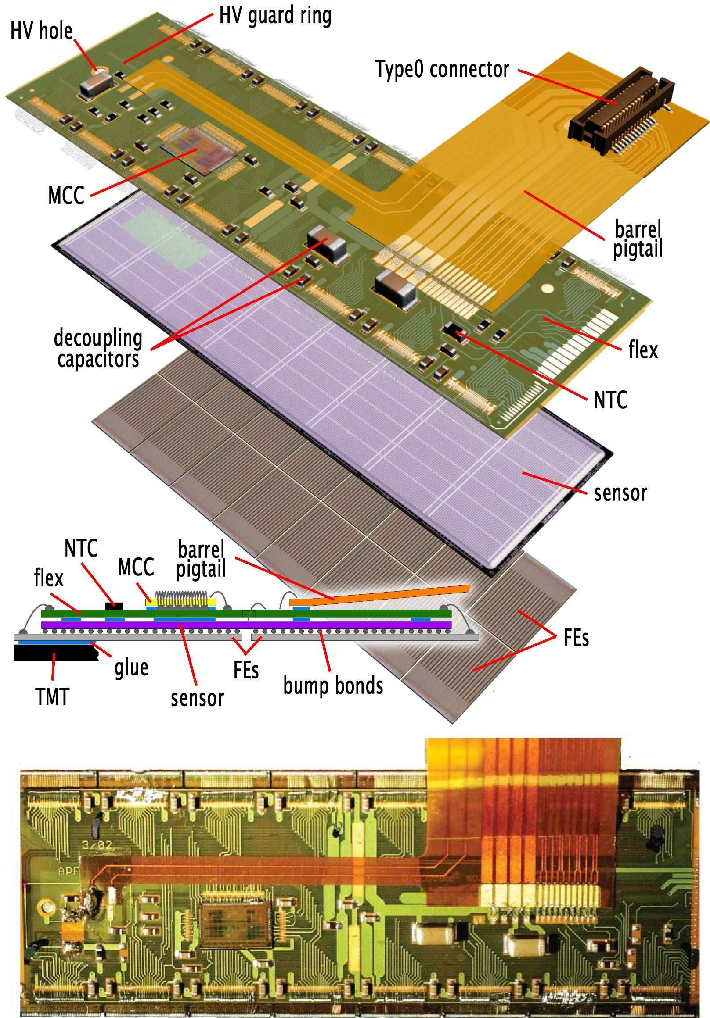
\includegraphics[width=6cm]{./pixel_detector.png}
\caption[ピクセルモジュールの全体像]{ピクセルモジュールの全体像\cite{1-2}。ピクセル検出器は、最小単位としてモジュールと呼ばれる構造を持ち、図はモジュールの全体像を示している。モジュールは、荷電粒子が通過し、信号を生成するセンサー部、AD変換を行うFEチップ部、データ転送等を行うフレキシブル基板から構成される。}
\label{pixel_detector}
\end{figure}

\subsubsection{ストリップ検出器}
ストリップ検出器はピクセル検出機の外側に設置されており、バレル部が4層、エンドキャップ部が18層となっている。
ストリップモジュールは、80$~\mu$mピッチのシリコンマイクロストリップセンサーを2枚重ねた構造をしている。
センサーの重ねる角度をずらすことによって、二次元の入射位置測定が可能となる。

\subsubsection{遷移放射検出器}
繊維放射検出器は内部飛跡検出器の最外層に設置される検出器であり、バレル部が73層、エンドキャップ部が320層で構成される。
この検出器はイオン化検出器であるドリフトチューブを重ねて構成される。
チューブの中心にはアノードとしてワイヤーが張られ、その周りは混合ガスで満たされている。
荷電粒子がドリフトチューブを通過すると、混合ガス中の分子をイオン化する。
発生した電子はチューブ内でドリフトし、これを収集することで電気信号を得る。

\subsection{カロリメータ}
カロリメータは内部飛跡検出器の外側に設置されている検出器であり、荷電粒子のエネルギー測定を行う。
主に電子・光子のエネルギー測定を目的とする電磁カロリメータと、ハドロンのエネルギー測定を目的とするハドロンカロリメータに分けられる。内側から電磁カロリメータ、ハドロンカロリメータの順に設置されている。
電子や光子が電磁カロリメータを通過する際、電子対生成や制動放射を繰り返し、電磁シャワーと呼ばれる粒子群となる。
このシャワーの合計エネルギーを取得することで、元の電子・光子のエネルギー測定を行う。
ハドロンカロリメータはハドロンのエネルギーを測定する。
ハドロンが通過すると、崩壊を繰り返し粒子シャワーを形成する。
この合計エネルギーを取得し、元のハドロンのエネルギー測定を行う。

\subsection{ミューオン検出器}
ミューオン検出器はATLAS検出機の最外層に設置されている。主にミューオンの検出を行い、その通過位置から運動量測定、そしてトリガー信号の生成を行う。
ミューオン検出器はガスで満たされたドリフトチューブを重ねて構成される。
ドリフトチューブを通過したミューオンはガス中の分子をイオン化する。
生成された電子をチューブ内のワイヤーで収集し、その到達時間からミューオンの通過位置を測定する。

\clearpage
\section{HL-LHC実験アップグレード計画}
LHCでは加速器のアップグレードを予定しており、これをHL-LHCアップグレード計画と呼ぶ。詳細を以下に示す。
\subsection{概要}
HL-LHCではルミノシティ\cite{1-13}を上げることで、衝突頻度を大きくし、取得統計数を増やす。
LHCとHL$-$LHCの比較を表\ref{compare_lhc}に示す。

\begin{table}[tbp]
\begin{center}
\caption[現行LHCとHL-LHCの比較]{現行LHCとHL-LHCの比較\cite{1-6}。瞬間ルミノシティは7倍、積分ルミノシティは10倍になることが見積もられており、取得統計数の増加が期待できる。}
\label{compare_lhc}
  \begin{tabular}{|lll|} \hline
    & LHC & HL$-$LHC \\ \hline
    重心系エネルギー & 14 & 14 \\
    瞬間ルミノシティ[$\rm{cm^{-2}s^{-1}}$] & $1\times 10^{34}$ & $7\times10^{34}$ \\
    積分ルミノシティ[$\rm{fb^{-1}}$] & $300$ & $3,000$ \\
    1バンチ交叉あたりの反応数 & $27$ & $140$ \\ \hline 
  \end{tabular}
\end{center}
\end{table}

LHCの運転計画を表\ref{hllhc_plan}に示す。
2025年の初めよりHL-LHCの導入が始まり、2027年の途中からHL-LHC運転開始の予定となっている。
\begin{figure}[bpt]\centering
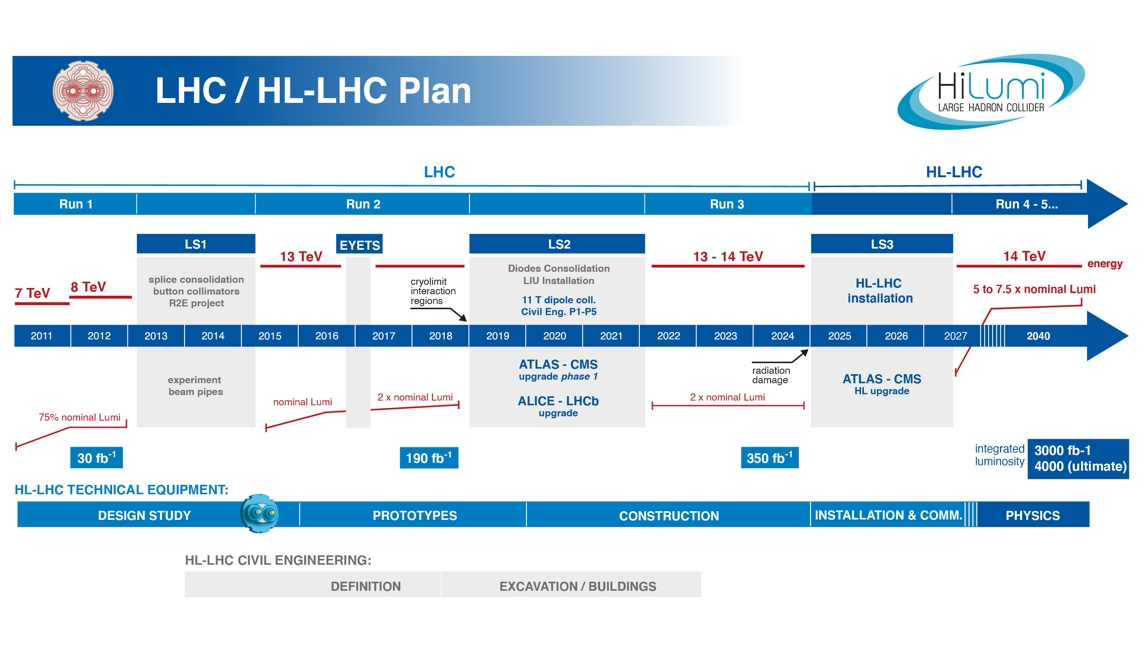
\includegraphics[width=12cm]{./hllhc_plan.jpg}
\caption[HL-LHC運転計画]{HL-LHC運転計画\cite{1-7}。2025年の初めよりHL-LHCの導入、2027年の途中より本運転が始まる。}
\label{hllhc_plan}
\end{figure}

\subsection{素粒子物理に対するモチベーション}
HL-LHCの素粒子物理に対するモチベーションに1つとして、ヒッグス粒子の性質の精密測定があげられる。
LHC、HL-LHCにおける粒子の質量とヒッグス粒子の結合定数の関係と統計誤差の見積もりをまとめたものを表\ref{higgs_uncertainty}に示す。
統計誤差が向上する見込みであり、より精密な標準模型の検証を行うことができる。

\begin{figure}[bpt]\centering
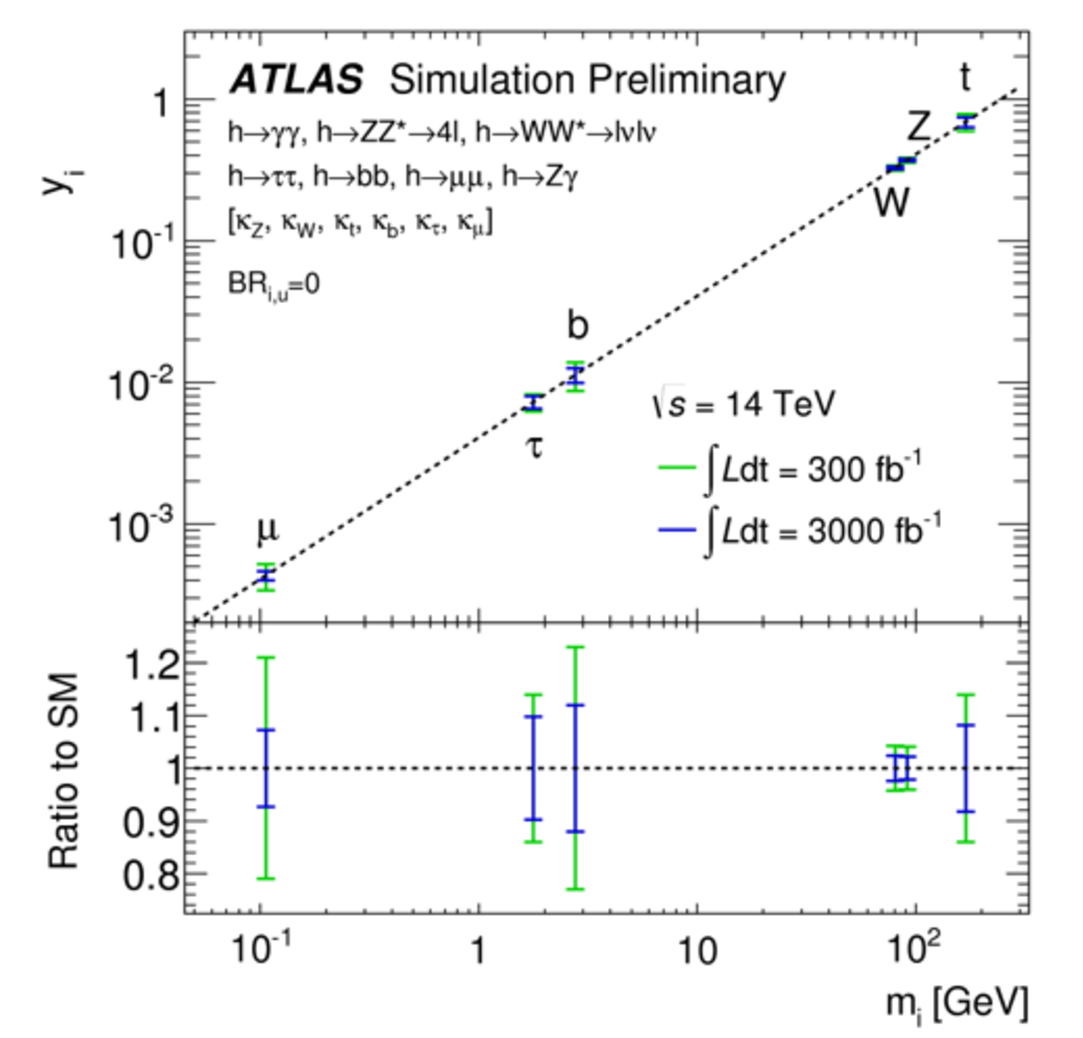
\includegraphics[width=10cm]{./higgs_uncertainty.pdf}
\caption[LHC、HL-LHCにおける粒子の質量とヒッグス粒子の結合定数の関係と統計誤差の見積もり]{LHC、HL-LHCにおける粒子の質量とヒッグス粒子の結合定数の関係と統計誤差の見積もり\cite{1-12}。図において青線、緑線がそれぞれLHC、HL-LHCの測定における統計誤差の見積もり値を示している。統計誤差は向上する見込みであり、標準模型の精密検証をすることができる。}
\label{higgs_uncertainty}
\end{figure}


\subsection{内部飛跡検出器のアップグレード}
HL-LHCのアップグレードによりルミノシティが増加するのに伴い、検出器には以下のような性能が要求される。

\begin{itemize}
  \item 放射線耐性の向上.\\
  統計量に伴い、放射線量も増加するため高放射線耐性が要求される。
  \item 高速読み出し.\\
  1バンチ交叉あたりの反応数(\textbf{パイルアップ})の増加に伴いトリガーレートが増加するため、現行よりも高速な読み出しが要求される。HLLHC運転時の最内層の検出器において、FEチップあたりの想定ヒット数は223.0、各ピクセルが持つヒット情報は4~bit、想定トリガーレートは1~MHzであり、FEチップを4枚搭載したモジュールでは$223.0\times 4 \times (1\times 10^6) \times 4 \simeq 4$~Gb/sの読み出しスピードが必要である。実際の要求値は5.12~Gb/sであり、現行の検出器のスピード160~Mb/sではこの要求を満たすことができない。
  \item 検出器の細密化.\\
  パイルアップが約5倍になるため、これらの衝突点を区別するためにはより細密な検出器を使用する必要がある。図\ref{detector_posi_res}にイメージを示す。
\end{itemize}

\begin{figure}[bpt]\centering
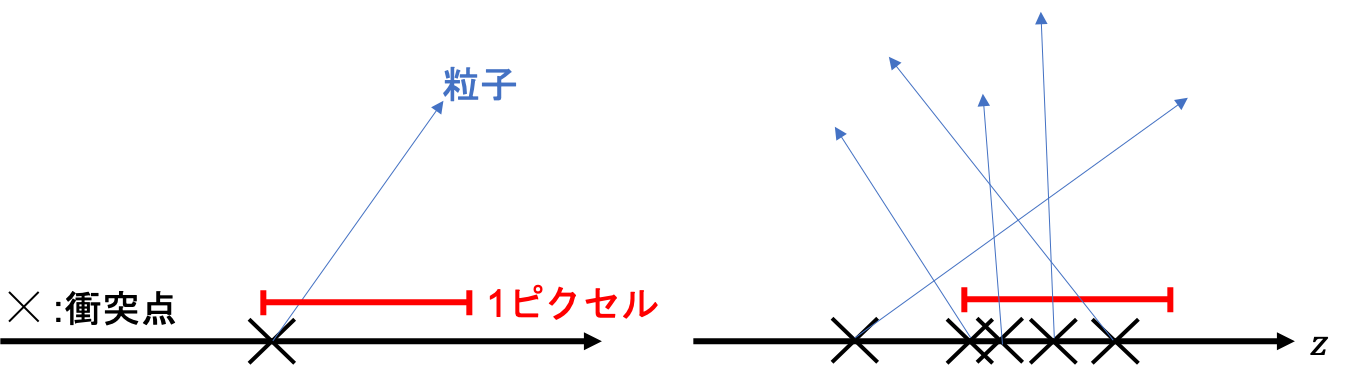
\includegraphics[width=12cm]{./detector_posi_res.png}
\caption[パイルアップ数増加のイメージ]{パイルアップ数増加のイメージ。図において青線が粒子、赤線が現行ピクセル検出器の1ピクセルの長さを示しており、$250~\mu$mである。左図がLHC、右図がHL-LHCの様子を表している。HL-LHCではパイルアップが約5倍に増えるため、図のように1交叉あたりの発生粒子数も増える。これらを区別し、精度良く粒子の衝突点を計算するには今までよりも細密な検出器を設置する必要がある。}
\label{detector_posi_res}
\end{figure}

HL-LHCに向けて内部飛跡検出器はアップグレードを予定しており、検出器の総入れ替えを行う。
アップグレード後の検出器を\textbf{Inner Tracker(ITk)}と呼ぶ。模式図を図\ref{itk_image}に示す。

\begin{figure}[bpt]\centering
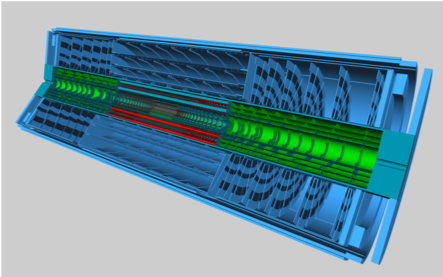
\includegraphics[width=10cm]{./itk_image.png}
\caption[ITkの全体像]{ITkの全体像\cite{1-3}。図はITk全体の模式図を示している。ITkはピクセル検出器(緑の領域)とストリップ検出器(青の領域)から構成される。}
\label{itk_image}
\end{figure}

\subsubsection{ITkの構成と現行ピクセル検出器との比較}
図\ref{itk_cross_section}にITkのビーム軸方向の断面図を示す。
ITkはピクセル検出器とストリップ検出器で構成される。
ピクセル検出器はバレル、傾斜バレル、エンドキャップ部で構成され、バレル部は5層となっている。

\begin{figure}[bpt]\centering
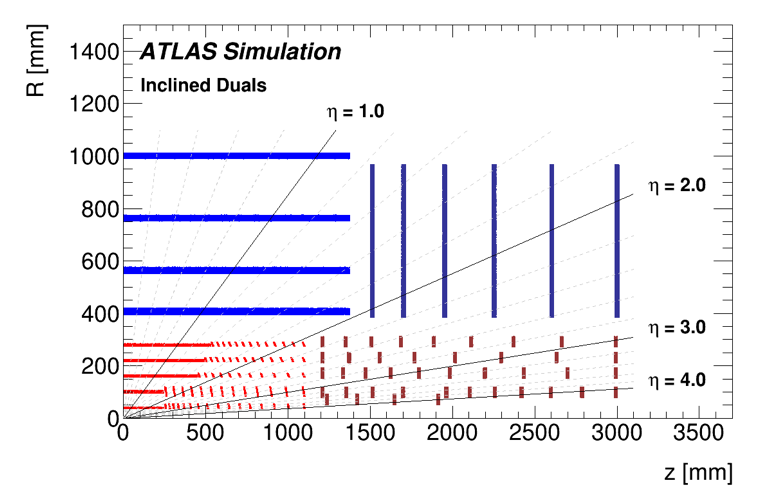
\includegraphics[width=12cm]{./itk_cross_section.png}
%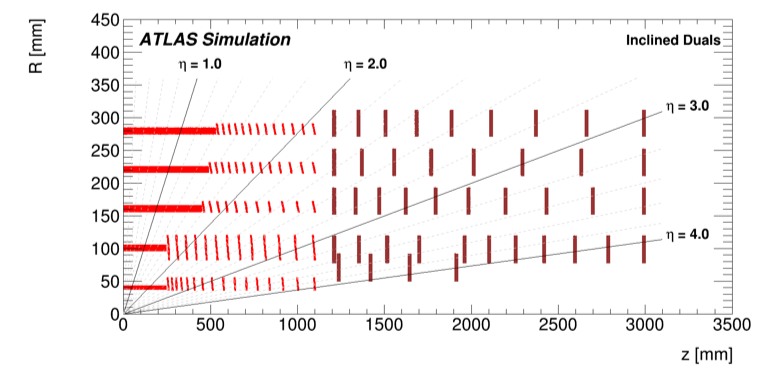
\includegraphics[width=10cm]{itk_pixel_cross_section}
\caption[ITkの断面図]{ITkの断面図\cite{1-3}。ITkはピクセル検出器とストリップ検出器から構成され、バレル部はそれぞれ5、4層の構造を持つ。ピクセル検出器はバレル部、傾斜バレル部、エンドキャップ部に分かれ、$|\eta|<4.0$までの範囲をカバーし、粒子の飛跡測定をすることができる設計となっている。}
\label{itk_cross_section}
\end{figure}

ピクセル検出器の配置に関して、現行とITkの比較を表\ref{compare_itk_pixel}に示す。
またモジュール数の比較を表\ref{compare_itk_modules}に示す。
ITkでは現行に比べ、$\eta$が大きい領域まで検出器を設置するため、その分使用するモジュール数も増える。

\begin{table}[tbp]
\begin{center}
\caption[ピクセル検出器設置領域の比較]{ピクセル検出器設置領域の比較。表は現行とITkにおけるピクセル検出器設置領域の比較を示す。$\eta$の範囲に関して、括弧内は度数法の値を示す。ITkでは遷移放射検出器を使用しないため、ピクセル検出器の半径方向のカバー領域が増え、層の数は4から5となる。また前方方向に生じる粒子測定を行うために、$\eta$の領域も拡大している。}
\label{compare_itk_pixel}
  \begin{tabular}{|lll|} \hline
    & 現行 & ITk \\ \hline
    $r[\rm{mm}]$ & $33〜129$ & $39〜279$ \\ 
    層の数(バレル部) & 4 & 5 \\ 
    $|\eta|$ & $<2.5~(<19^\circ)$ & $<4~(<4.2^\circ)$ \\ \hline
  \end{tabular}
\end{center}
\end{table}

\begin{table}[tbp]
\begin{center}
\caption[搭載するピクセルモジュール数の比較]{搭載するピクセルモジュール数の比較。表は現行とITkのピクセル検出器において、各構造における搭載ピクセルモジュールの数を示している。傾斜バレル部、エンドキャップ部はリングと呼ばれる構造が$z$軸方向に層になっており、括弧内の数字は各層におけるリング構造の数を示す。ITkではバレル部で現行の約2倍になっているのに加え、傾斜バレル部、エンドキャップ部に多くのモジュールを搭載する設計となっていることが分かる。}
\label{compare_itk_modules}
  \begin{tabular}{|l||ll|ll|ll|} \hline
          & バレル部 &            & 傾斜バレル部 & & エンドキャップ部 & \\ \hline 
    層    & 現行     & ITk        & 現行& ITk          & 現行     & ITk \\ \hline
    1     & $280$    & $192$      & $-$ & $512(32)$        & $-$      & $64(8)$ \\ 
    2     & $286$    & $240$      & $-$ & $520(26)$        & $-$      & $242(22)$ \\ 
    3     & $494$    & $660$      & $-$ & $660(22)$        & $-$      & $320(20)$ \\ 
    4     & $676$    & $960$      & $-$ & $1040(26)$       & $288(6)$ & $352(16)$ \\ 
    5     & $-$      & $1300$     & $-$ & $1300(26)$       & $-$      & $468(18)$ \\ \hline
    合計  & $1736$   & $3352$     & $0$ & $4032$       & $288$    & $1446$ \\ \hline\hline
  \end{tabular}
\end{center}
\end{table}

\clearpage
\subsection{物理測定に及ぼす影響}
カバーする$\eta$の範囲が大きい特徴が生む利点として、前方方向に大きな運動量を持つ粒子を含む物理イベントの測定精度向上があげられる。

この例として、ボゾン粒子結合によるヒッグス粒子生成過程(Vector boson fusion higgs production, \textbf{VBF})をあげる。
VBFの1つのチャンネルに関するファインマン図及びイベントディスプレイを図\ref{VBF_image}に示す。
この衝突により生じる2つのクオークはジェットと呼ばれる粒子群となり、多くのジェットは図\ref{VBF_jet_eta}に示すように前方方向に大きな運動量を持つ。

現行ATLAS検出器のカロリメータでは$|\eta|<4.9$の領域をカバーしている。
ITkでは、飛跡検出器でジェットを捉えることによってエネルギーや崩壊点測定精度の向上が期待され、
VBFイベントの測定精度を向上することができる。

$VBF~H\rightarrow WW$における系統誤差は表\ref{VBF_uncertainty}のように見積もられる\cite{1-3}。

\begin{figure}[bpt]
  \begin{minipage}{0.5\hsize}
    \begin{center}
    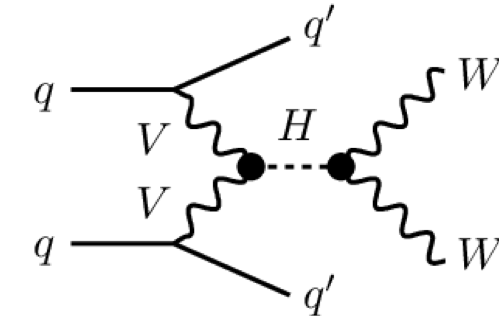
\includegraphics[width=70mm]{./VBF_fainman.png}
    \end{center}
  \end{minipage}
  \begin{minipage}{0.5\hsize}
    \begin{center}
    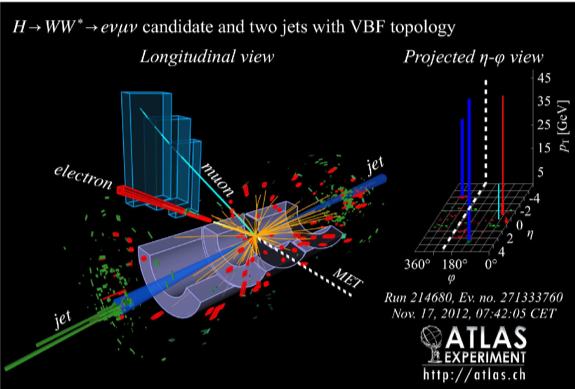
\includegraphics[width=70mm]{./VBF_event_display.png}
    \end{center}
  \end{minipage}
  \caption[VBFイベントの図]{VBFイベントの図\cite{1-8}。図はVBFイベントの一つである$H\rightarrow WW$崩壊チャンネルを示している。左図はファインマン図、右図はそのイベントディスプレイを表す。このイベントにおいて、初めに相互作用したクオーク対は、それぞれハドロン化しジェットと呼ばれる粒子群となる。このときこれらのジェットは前方方向に大きな運動量を持つ。ITkでは$|\eta|<4.0$の範囲をカバーしており、このようなジェットを捉えることができるため、測定精度が向上する。}
  \label{VBF_image}
\end{figure}

\begin{figure}[bpt]\centering
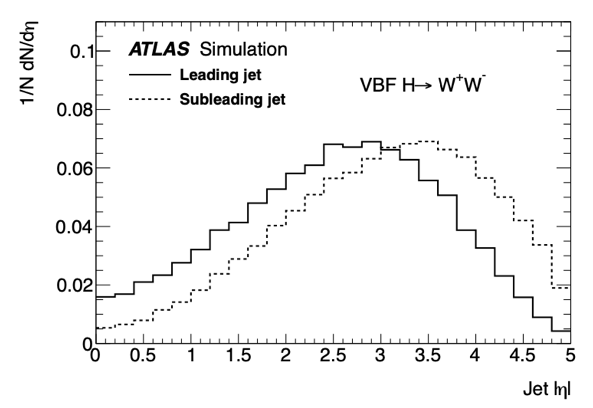
\includegraphics[width=8cm]{./VBF_jet_eta.png}
\caption[VBFイベントにおけるジェットの運動方向の$\eta$分布]{VBFイベントにおけるジェットの運動方向の$\eta$分布\cite{1-3}。図はシミュレーションの結果を示している。横軸はジェットの運動方向の$\eta$成分を示しており、縦軸はイベント数に比例する量である。``Leading jet"、``Subleading jet"は各イベントにおいて1、2番目に大きな運動量を持つジェットである。$|\eta|=3-3.5$付近にピークを持ち、多くのジェットは前方方向に大きい運動量を持つことが分かる。}
\label{VBF_jet_eta}
\end{figure}

\begin{table}[bpt]
\begin{center}
\caption[VBF~$H\rightarrow WW$の測定における系統誤差の見積もり]{VBF~$H\rightarrow WW$の測定における系統誤差の見積もり\cite{1-3}。表は3000~$\rm{fb^{-1}}$において、$|\eta| <2.7$、$|\eta| <4.0$の領域を使用した場合のVBF~$H\rightarrow WW$イベント測定における系統誤差の見積もりを示している。$|\eta| <4.0$の領域を使用することで系統誤差が向上する見積もりであることが分かる。ここでは統計誤差は考慮にいれていない。}
\label{VBF_uncertainty}
  \begin{tabular}{|lll|} \hline
    検出器の使用範囲 & $|\eta| <2.7 $ & $|\eta| < 4.0 $ \\ \hline
    系統誤差 & 22$\%$ & 12$\%$ \\ \hline
  \end{tabular}
\end{center}
\end{table}

